% ===== 分片 A：引言 + §1 标题与导语 + §1.1–§1.4（原文 PDF 第 2–9 页）=====
\section*{引言}
\addcontentsline{toc}{section}{引言}

\begin{keypoints}
\begin{itemize}
  \item \textbf{物理图像：}本讲义围绕 Seiberg 与 Witten 关于 $N=2$ 超对称量子色动力学（SQCD）精确结果的工作展开，读懂它需要预先备齐磁单极与超对称两块背景。
  \item \textbf{数学工具：}狄拉克磁单极与电荷量子化 $\to$ 't Hooft–Polyakov 磁单极与 Bogomol'nyi 界 $\to$ $N=1,2$ 超对称拉格朗日量与中心荷 $\to$ 模空间上的单值变换、完全椭圆积分与对偶。
  \item \textbf{关键结论：}全文分四节：§1 规范场论中的磁单极；§2 超对称规范理论；§3 $N=2$ 纯规范理论的 Seiberg–Witten 分析；§4 含物质场的推广。更完整的文献指引见 \cite{Lerche}。
\end{itemize}
\end{keypoints}

本讲义是 1995 年在意大利的里雅斯特（Trieste）暑期学校所作一系列讲座的书面整理稿，其成文远晚于讲座本身。讲座的目的是对 Seiberg 与 Witten 关于量子色动力学的 $N=2$ 超对称扩充之精确结果的工作，给出一个基础性的介绍。我们希望把深入研究其工作所需的全部背景材料集中在一处。我们设想的读者是已经修过量子场论课程的研究生，除此以外并不期望读者具备更多的背景知识就能跟上这些讲座。我们已尽力使讲解循序渐进、便于教学。在某些小节中，我们大量借用了已有的综述：例如在超对称的处理上我们遵循 Bagger 与 Wess \cite{WB}，在磁单极理论中则采用了 Goddard 与 Olive \cite{GO} 以及 S. Coleman \cite{coleman1,coleman2} 的综述。这些文献对这些课题给出了出色的阐述，我们也没有非要改进其讲述的充分理由。同样显而易见的是，我们大量引用了 Seiberg 与 Witten 的原始论文 \cite{SW-I,SW2}，但我们力图提供必要的工具，使有兴趣的学生和/或研究者更容易读懂这些论文。近来还出版了若干水平更高的讲义，其中可以找到更多细节以及与弦论的联系（例如可参见 W. Lerche 的讲义 \cite{Lerche}）。我们还想说明，我们并未试图穷尽地引用该课题的全部文献；更完整的参考文献列表可在 \cite{Lerche} 中找到。本文的文献列表意在为进入弦论与场论中对偶性这一迅速增长的文献提供入门指引。对于因未能列入其工作而可能感到不快的作者，我们深表歉意。

% [Tutor Note: 见原文 PDF 第 2 页引言第一段。文中“Trieste Summer School”指 1995 年在意大利的里雅斯特（Trieste）举办的暑期学校系列讲座，本讲义即这些讲座的整理稿；原文称其为“very late written version”（很晚才写成的版本），故译作“成文远晚于讲座本身”。]

本讲义分为四节，每一节又进一步细分为若干小节。第 1 节介绍规范场论中的磁单极。我们先讨论狄拉克磁单极与电荷量子化的思想，然后描述具有自发对称性破缺的规范理论中的 't Hooft–Polyakov 磁单极。随后我们引入 Bogomol'nyi 界与 BPS 态的概念。在此之后，我们描述磁单极的拓扑分类，然后叙述电磁对偶的 Montonen–Olive 猜想。本节最后，我们说明当拉格朗日量中存在 $\theta$ 项时，磁单极的电荷会因其磁荷而发生平移。第 2 节介绍超对称规范理论。我们首先描述超对称代数，以及它不含中心荷与含中心荷的表示，并讨论它在超场语言下的局域实现。然后构造 $N=1$ 的拉格朗日量，最后构造同时含规范多重态与物质多重态（超多重态）的 $N=2$ 超对称拉格朗日量。在本节末尾，我们分别在纯规范理论与含物质的理论中计算 $N=2$ 中心荷，并确立它与 BPS 界的关系。在前两节建立基础之后，第 3 节描述对规范群为 $SU(2)$ 的 $N=2$ 纯规范理论所作的 Seiberg–Witten 分析。在前两个小节中，我们讨论模空间的参数化与 $R$ 对称性的破缺。接着说明如何利用该理论的手征 $U(1)$ 反常得到低能有效作用量的单圈形式。本节其余部分则致力于借助对偶性以及理论模空间上的奇点结构求出精确的低能有效作用量。我们用完全椭圆积分表示这一精确解。在第 4 节中，我们简要描述对含 $N_f$ 个物质场的 $N=2$ $SU(2)$ 规范理论所作的 Seiberg–Witten 分析。在讨论这类理论的一般特征之后，我们说明其（对偶）群不再单纯是 $SL(2,Z)$。然后描述这些理论模空间上的奇点结构，并勾勒求得精确解的步骤。第 4 节的目的只是让读者对含物质理论的分析有所体会；若要更深入的理解，有兴趣的读者可参阅 Seiberg 与 Witten 的原始工作。

% [Tutor Note: 见原文 PDF 第 3 页引言第二段。原文称含物质时“the duality group is no longer pure $SL(2,Z)$”，其中“pure”指对偶群不再是整个 $SL(2,Z)$，而是它的真子群（同余子群）；具体形式与物质场的味数 $N_f$ 有关，详见原文第 4.6 节（原文 PDF 第 75 页起）。]

\section{规范场论中的磁单极}

\begin{keypoints}
\begin{itemize}
  \item \textbf{物理图像：}磁单极在规范场论中作为孤立子（拓扑缺陷）出现；'t Hooft–Polyakov 磁单极是 $SO(3)$ 规范理论经希格斯机制自发破缺到 $U(1)$ 后的非微扰态。
  \item \textbf{数学工具：}狄拉克弦与电荷量子化条件（式(\ref{XII})、(\ref{DSZ})）；磁单极的拓扑分类（同伦群）；Bogomol'nyi 界与 BPS 饱和。
  \item \textbf{关键结论：}$SO(3)$ Georgi–Glashow 模型的微扰谱为有质量希格斯粒子 $H$、光子 $\gamma$ 与 $W^\pm$ 玻色子，其非微扰谱中还包含磁单极与双子。
  \item \textbf{本节路线：}§1.1 约定与预备知识；§1.2 电荷量子化的半经典推导；§1.3 狄拉克弦；§1.4 Georgi–Glashow 模型。§1.5 之后的单极解、Bogomol'nyi 界、Montonen–Olive 猜想与 $\theta$ 项效应见后续小节。
\end{itemize}
\end{keypoints}

本节我们先回顾狄拉克磁单极的性质与电荷量子化的思想。然后描述具有自发对称性破缺的非阿贝尔规范理论中出现的磁单极与双子，并讨论它们的一般性质。我们还引入 Bogomol'nyi 界与 BPS 态的概念。在最后两个小节中，我们描述电磁对偶的 Montonen–Olive 猜想，以及 Witten 关于拉格朗日量中 $\theta$ 项的存在如何改变磁单极与双子电荷的论证。关于本节大部分材料更详细的讨论，读者可参阅 Goddard 与 Olive 的综述文章 \cite{GO}，以及 Coleman 的讲义 \cite{coleman1,coleman2}。

\subsection{约定与预备知识}

我们先陈述约定：我们始终取 $c=1$，并且几乎总取 $\hbar=1$，除非需要区分经典效应与量子效应。处理指标升降时，我们使用号差为 $\{ +,-,-,-\}$ 的平直 Minkowski 度规 $\eta$。此外，我们选取使麦克斯韦方程组取如下形式的单位：
\begin{equation}
\begin{array}{l}
\vec{\nabla}\cdot\vec{E}=\rho\,,\qquad\vec{\nabla}\times\vec{B}-
\partial \vec{E}/\partial t =\vec{j}\,,\\
\vec{\nabla}\cdot\vec{B}=0\,,\qquad \vec{\nabla}\times\vec{E} +
\partial\vec{B}/\partial t = 0\,.
\label{I}
\end{array}
\end{equation}
在这些单位下，库仑定律中出现因子 $(4 \pi)^{-1}$：对于位于原点的静态点状电荷 $q$，有 $\rho = q 
\delta^{3}(\vec{r})$。将第一个麦克斯韦方程在半径为 $r$ 的球面上积分并利用球对称性，得到
$\int_{S^2} \vec{E} \cdot d \vec{s}=4\pi r^2 E(r)=q$。因此，如前面所说，
$\vec{E}=q\vec{r}/4\pi r^{3}$。由 $\vec{E}=-\vec{\nabla}\phi$ 定义的静电势 $\phi$ 为
$\phi = q / 4 \pi r$。

% [Tutor Note: 见原文 PDF 第 3 页式 (1)。此处采用的是 $c=\hbar=1$ 且库仑定律带因子 $(4\pi)^{-1}$ 的“有理化”单位制（Lorentz–Heaviside 型），故点电荷场强为 $\vec{E}=q\vec{r}/4\pi r^{3}$ 而非 $q\vec{r}/r^{3}$。后文的 $4\pi$、$e=q/\hbar$ 以及磁荷 $g$ 的归一化全都由它确定；若换用 SI 或高斯制，电荷量子化条件会整体差一个 $4\pi$，核对时请务必以此单位制为准。]

在相对论记法中，引入四维势 $A^{\mu}= \{\phi, \vec{A}\}$。电场与磁场定义为相应场强张量 $F_{\mu\nu}$ 的分量，具体如下：
\begin{eqnarray}
F_{\mu \nu} & = &\partial_{\mu}A_{\nu} - \partial_{\nu}A_{\mu}\,,
\nonumber \\
F_{0i} & = &\partial_{0}A_{i} - \partial_{i}A_{0} =
- \partial_{0}A^{i} - \partial_{i}A^{0} = E^{i}\,,\nonumber \\
F_{ij} & = & \partial_{i}A_{j} - \partial_{j}A_{i} =
- (\partial_{i}A^{j} - \partial^{j}A_{i}) =
-\epsilon_{ijk} B^{k}\,,
\label{III}
\end{eqnarray}
于是 $B^i=-\frac{1}{2}\epsilon^{ijk}F_{jk}=-\frac{1}{2}
\epsilon^{oi\mu\nu}F_{\mu\nu}$。对偶场强张量由下式给出
$$
\widetilde F^{\mu \nu} = \frac{1}{2} \varepsilon^{\mu \nu \alpha
\beta} F_{\alpha \beta}\,,
$$
其中 $\varepsilon^{0123}=+1$。用分量记法，我们有
\begin{equation}
F^{\mu \nu} =
\left(
\begin{array}{cccc}
0 & -E_{x} & -E_{y} & -E_{z}  \\
E_{x} & 0 & -B_{z} & B_{y} \\
E_{y} & B_{z} & 0 & -B_{x} \\
E_{z} & -B_{x} & B_{y} & 0
\end{array}
\right)\,,
\qquad
\widetilde F^{\mu \nu} =
\left(
\begin{array}{cccc}
0 & -B_{x} & -B_{y} & -B_{z} \\
B_{x} & 0 & E_{z} & -E_{y} \\
B_{y} & -E_{z} & 0 & E_{x} \\
B_{z} & E_{y} & -E_{x} & 0
\end{array}
\right)\,.
\label{IV}
\end{equation}

% [Tutor Note: 见原文 PDF 第 3 页式 (2) 与第 4 页式 (3)。在号差 $(+,-,-,-)$、$\varepsilon^{0123}=+1$ 下，$F_{0i}=E^i$ 但升指标得 $F^{0i}=-E^i$，同理 $\widetilde F^{0i}=-B^i$；式 (3) 的两个矩阵里 $E$、$B$ 的符号分布正是这一约定的结果，此处是最容易漏掉负号的地方，请逐项核对。]

用电四维流 $j^{\mu}=\{\rho,\vec{j}\}$ 表示，麦克斯韦方程组取紧凑形式
\begin{equation}
\partial_\nu F^{\mu\nu}=-j^\mu\,,\qquad\partial_\nu\,\widetilde
F^{\mu\nu}=0\,. \label{V}
\end{equation}
注意当 $j^\mu =0$ 时，上述方程在替换 $\vec{E} \rightarrow \vec{B}, \vec{B} \rightarrow
-\vec{E}$ 下不变。这称为电磁对偶变换。当存在电源时，该变换不再是麦克斯韦方程组的对称性。为了使这些方程在 $j^{\mu}$ 非零时恢复对偶不变性，Dirac \cite{Dirac} 引入了磁四维流 $k^{\mu}=\{\sigma ,\vec{k}\}$，并把麦克斯韦方程组修改为
\begin{equation}
\partial_\nu F^{\mu\nu}=-j^\mu\,,\qquad\partial_\nu\,
\widetilde F^{\mu\nu}= -k^\mu \,.   
\label{VI}
\end{equation}
现在上述方程在场与流的联合对偶变换下不变，该变换可写为
\begin{equation}
F\rightarrow \widetilde F\,,\,\widetilde F\rightarrow-F\,;\qquad 
j^\mu\rightarrow k^\mu\,,\, k^\mu\rightarrow -j^\mu\,.
\label{emduality}
\end{equation}
注意方程组(\ref{VI})的完全不变群比这个离散对偶变换更大。事实上，它们在一个连续的 $SO(2)$ 群下不变，该群把电学量与磁学量相互旋转。

% [Tutor Note: 见原文 PDF 第 4 页式 (5)、(6)。要点有二：其一，对偶不变性只在场与流“同时”按式 (6) 变换时才成立，单独变换场并不是麦克斯韦方程组的对称性；其二，原文所说连续的 $SO(2)$ 群指 $(F,\widetilde F)$ 平面内的转动（等价于对复组合 $F+i\widetilde F$ 作相位变换），这正是后文 $S$ 对偶连续版本的雏形。]

对于点状电源与点状磁源，流密度可写为
\begin{eqnarray}
j^{\mu}(x) & = & \sum_{a} q_{a} \, \int \, dx_{a}^{\mu}
\delta^{4} (x - x_{a})\,, \nonumber \\
k^{\mu}(x) & = & \sum_{a} g_{a} \, \int \, dx_{a}^{\mu}
\delta^{4} (x - x_{a})\,.\nonumber
\end{eqnarray}
带有电荷 $q$ 与磁荷 $g$ 的粒子受到如下洛伦兹力：
$$
m\,\frac{d^2x^\mu}{d\tau^2}=(q F^{\mu\nu}+g\, \widetilde F^{\mu\nu})
\frac{dx_\nu}{d\tau}\,.
$$

尽管在运动方程的层面上，Dirac 对麦克斯韦理论的修改似乎无关紧要，但它在量子理论中有着极为非平凡的后果。认识这一问题的一个途径是注意到，在理论的量子表述中矢量势 $\vec{A}$ 是不可或缺的；另一方面，方程
$\vec{B}=\vec{\nabla}\times \vec{A}$ 与 $\vec{\nabla}\cdot\vec{B}\ne
0$ 并不相容，除非矢量势 $\vec{A}$ 带有奇点，因而并非整体良定义。结果表明，这些奇点依赖于规范选择，因此它们的存在不应当在实验上可观测。在可以仅用 $\vec B$ 表述的经典理论中，这一要求平凡地得到满足。然而在量子理论中，它导致了电荷量子化这一重要现象。下面我们先给出这一效应的半经典推导，然后描述基于狄拉克弦概念的推导。
 
\subsection{电荷量子化的半经典推导}

考虑一个非相对论性电荷 $q$，位于原点处强度为 $g$ 的磁单极附近。电荷 $q$ 受到力 $m\ddot{\vec{r}}=q\dot{\vec{r}}\times\vec{B}$，其中 $\vec{B}$ 是由 $\vec{B}= 
g\vec{r}/4\pi r^3$ 给出的磁单极场。在该力作用下，电荷的轨道角动量的变化由下式给出
$$
\frac{d}{dt}\left(\,m\vec{r}\times\dot{\vec{r}}\right) =
m\vec{r}\times\ddot{\vec{r}}= \frac{qg}{4 \pi r^{3}}\,
\vec{r}\times\left(\dot{\vec{r}}\times\vec{r}\right)= 
\frac{d}{dt}\left(\frac{qg}{4\pi}\,\frac{\vec{r}}{r}\right)\,.
$$
因此，系统的总守恒角动量为
\begin{equation}
\vec{J}=\vec{r}\times m\dot{\vec{r}}-\frac{qg}{4\pi}\,
\frac{\vec{r}}{r}\,.
\label{XI}
\end{equation}
右端第二项（以下记作 $\vec{J}_{em}$）是来自电磁场的贡献。这一项可以直接计算：电磁场的动量密度由其坡印廷矢量 $\vec{E}\times\vec{B}$ 给出，因此它对角动量的贡献为
$$
\vec{J}_{em} = \int \, d^{3}x \, \vec{r} \times
(\vec{E} \times \vec{B}) = \frac{g}{4 \pi} \,
\int \, d^{3} x \, \vec{r} \times
\left( \vec{E} \times \frac{\vec{r}}{r^{3}} \right)\,.
$$
写成分量，
\begin{eqnarray}
J^i_{em} & = & \frac{g}{4 \pi} \, \int \, d^{3}x E^{j}
\left( \delta_{ij} - \frac{x_i x_j}{r^{2}} \right )
\frac{1}{r} = \frac{g}{4 \pi} \, \int \, d^{3}x E^{j}
\partial_{j} (\hat{x}^{i}) \nonumber \\
& = & \frac{g}{4 \pi} \int_{S^2} \hat{x}^i \vec{E}\cdot \vec{ds} 
- \frac{g}{4 \pi} \, \int \, d^{3}x \vec{\nabla} \cdot
\vec{E} \hat{x}^{i}\,. 
\label{XIV}
\end{eqnarray}
当电、磁荷之间的距离与它们到边界 $S^2$ 的距离相比可以忽略时，第一个积分对 $\vec{J}_{em}$ 的贡献因球对称性而消失。于是只剩下
\begin{equation}
\vec{J}_{em}= -\frac{gq}{4 \pi} \hat{r}
\label{Jem}\,.
\end{equation}

% [Tutor Note: 见原文 PDF 第 5 页式 (8)。第二个等号是分部积分：$\partial_j\hat{x}^i=(\delta_{ij}-x_ix_j/r^2)/r$，再把 $E^j\partial_j\hat{x}^i$ 写成 $\partial_j(E^j\hat{x}^i)-\hat{x}^i\partial_j E^j$。原文只说“球对称使第一个积分消失”，对真正给出式 (9) 的 $\vec{\nabla}\cdot\vec{E}=q\delta^{3}(\vec{r})$ 一项轻轻带过——恰恰是原点处的 $\delta$ 源贡献了 $-qg/4\pi\,\hat{r}$。这是本段最容易“差一个符号”的地方，请按 $\partial_j\hat{x}^i$ 的符号重新核对。]

回到式(\ref{XI})，若假设轨道角动量是量子化的，则由此可得
\begin{equation}
\frac{qg}{4 \pi} = \frac{1}{2} n \hbar\,,
\label{XII}
\end{equation}
其中 $n$ 为整数。注意在上面的推导中，我们假设了电荷–磁单极系统的总角动量以半整数倍为单位量子化。考虑到我们并不需要把带电粒子或磁单极当作费米子，这是一个奇怪的假设：两个组分都是玻色子。然而结果表明情形确实如此，而且这种情形并不违反自旋–统计定理
\cite{Goldhaber,Wilczek}。我们不再进一步讨论这一问题，但要指出，下一小节给出的同一方程的推导并不依赖于这一假设。

% [Tutor Note: 见原文 PDF 第 6 页式 (10) 前一句。原文“if we assume that orbital angular momentum is quantized. Then it follows that”在句号处应作逗号（原文标点笔误），译文的句式已按正确逻辑重写。物理上这里假设的是“总角动量（含场角动量 $\vec{J}_{em}$）以 $n\hbar/2$ 量子化”，而非纯轨道角动量；随后原文承认这与两个组元都是玻色子相矛盾，并把解释归于文献 [5,6]（Goldhaber、Wilczek）。下一小节由狄拉克弦给出的推导不依赖此假设。]

式(\ref{XII})就是狄拉克电荷量子化条件。它意味着：如果宇宙中某处存在一个磁荷为 $g$ 的磁单极，那么所有电荷都以 $2\pi\hbar/g$ 为单位量子化。如果我们有若干纯电荷 $q_i$ 和若干纯磁荷 $g_j$，那么它们中任意一对都满足一个量子化条件：
\begin{equation}
\frac{q_{i}g_{j}}{4 \pi \hbar} = \frac{1}{2} n_{ij}
\label{XIII}
\end{equation}
因此，任何电荷都是 $2\pi\hbar/g_j$ 的整数倍。对给定的 $g_j$，设这些电荷的最大公因子为 $n_{0j}$。那么所有电荷都是 $q_{0}=n_{0j}2\pi\hbar /g_{j}$ 的倍数。注意 $q_0$ 本身未必存在于谱中。类似的考虑也适用于磁荷的量子化。

到目前为止，我们只处理了或者带电荷、或者带磁荷的粒子。现在我们考虑双子，即同时携带电荷与磁荷的粒子。考虑两个双子，其荷分别为 $(q_1,g_1)$ 与 $(q_2,g_2)$。对该系统，我们可以按(\ref{XIV})中的步骤重复 $\vec{J}_{em}$ 的计算，只是现在电磁场要分解为 $\vec{E}=\vec{E}_1+\vec{E}_2$ 与 $\vec{B}=\vec{B}_1+ \vec{B}_2$。容易求得结果为

\begin{equation}
\vec{J}_{em}=-\frac{1}{4\pi}\left(q_1 g_2 - q_2 g_1\right)\hat{r} 
\label{Jemd}
\end{equation}
于是电荷量子化条件推广为
\begin{equation}
\frac{q_1 g_2 - q_2 g_1}{4\pi\hbar}=\frac{1}{2} n_{12}
\label{DSZ}
\end{equation}
这称为 Dirac–Schwinger–Zwanziger 条件
\cite{Schwinger,Zwanziger}。该条件在 $SO(2)$ 变换 $(q+ig)\rightarrow e^{i\phi}(q+ig)$ 下不变，而后者也是(\ref{VI})的一个对称性。

% [Tutor Note: 见原文 PDF 第 6 页式 (13)。注意 $n_{12}$ 依赖两粒子的编号顺序，交换 $1\leftrightarrow2$ 时 $n_{12}\to-n_{12}$；而 $q_1g_2-q_2g_1$ 正是二维矢量 $(q_i,g_i)$ 的行列式，在 $(q_i,g_i)$ 整体 $SO(2)$ 转动下不变。这一“量子化条件与连续对偶相容”的事实，正是后文（§4）把对偶群视为 $SL(2,Z)$ 的子群、并研究其单值变换的出发点。]

\subsection{狄拉克弦}

下面我们给出狄拉克量子化条件的更严格推导，它基于狄拉克弦这一概念。用 $\vec{B}_{mon}$ 表示磁单极周围的磁场。由于 $\vec{\nabla}\cdot\vec{B}_{mon}\ne 0$，不可能构造一个良定义的 $\vec{A}_{mon}$ 使得
$\vec{B}_{mon}=\vec{\nabla} \vec{A}_{mon}$。为克服这一困难，Dirac 引入了一根半无限长的螺线管（或弦），它从 $(0,0,-\infty)$ 延伸到磁单极所在的位置 $(0,0,0)$。该螺线管携带磁场 $\vec{B}_{sol}=g\theta (-z)\delta(x)
\delta(y)\hat{z}$，它同样不是无散的。然而，总磁场
\begin{equation}
\vec{B}=\vec{B}_{mon}+\vec{B}_{sol}=\frac{g}{4\pi r^{2}}+g\theta(-z)
\delta(x)\delta(y)\hat{z}\,,
\end{equation}
满足 $\vec{\nabla}\cdot\vec{B}=g\delta(\vec{r})-g\delta(\vec{r}) 
=0$。因此，可以为磁单极–螺线管系统构造一个非奇异的 $\vec{A}=
\vec{A}_{mon}+\vec{A}_{sol}$。事实上，与狄拉克弦相联系的奇异 $\vec{A}_{sol}$ 正是用来抵消 $\vec{A}_{mon}$ 中的奇性的。$\vec{A}_{mon}$ 中奇点的位置、从而狄拉克弦的位置，可以通过奇异规范变换移动。既然狄拉克弦是人为构造的，它就应当是不可观测的，也不应对任何物理过程有贡献。然而，在 Aharonov–Bohm 实验中，弦的存在会通过对其相位的贡献影响电荷的波函数。沿一条环绕该弦、并围出面积 $S$ 的回路 $\Gamma$，由此得到的 Aharonov–Bohm 相位容易算出为
$$
e \oint_{\Gamma} \vec{A}_{sol} \cdot d \vec{l} = e \int_S
\vec{B}_{sol} \cdot d\vec{s} = e g\,.
$$
这里，$e=q/\hbar$ 是电磁耦合常数。只要
$$
e g = 2\pi n\,,
$$
该相位、从而狄拉克弦便是不可观测的，这再次给出狄拉克电荷量子化条件。

% [Tutor Note: 见原文 PDF 第 7 页第 2 行。原文写 $\vec{B}_{mon}=\vec{\nabla} \vec{A}_{mon}$，漏掉叉乘号，应为 $\vec{B}_{mon}=\vec{\nabla}\times\vec{A}_{mon}$（原文笔误，译文照录）。正因为磁单极场满足 $\vec{\nabla}\cdot\vec{B}_{mon}\ne 0$，这样的 $\vec{A}_{mon}$ 才无法整体存在。]

% [Tutor Note: 见原文 PDF 第 7 页式 (14)。其中 $g/4\pi r^{2}$ 一项应为 $g\hat{r}/4\pi r^{2}$（即 $\vec{B}_{mon}=g\vec{r}/4\pi r^{3}$），原文漏写单位矢量 $\hat{r}$（原文笔误，译文照录）；补上它，$\vec{B}_{mon}$ 的方向信息才完整，也才能与 $\vec{\nabla}\cdot\vec{B}_{mon}=g\delta^{3}(\vec{r})$ 自洽。]

% [Tutor Note: 见原文 PDF 第 7 页“Aharonov–Bohm 相位”一段，紧接式 (14) 之后。相位 $e\oint_\Gamma\vec{A}_{sol}\cdot d\vec{l}=eg$ 中的 $e$ 是经 $\hbar$ 归一化的耦合常数 $e=q/\hbar$（原文如此，并非裸电荷），故 $eg=2\pi n$ 与上小节的 $qg/4\pi\hbar=n/2$ 完全等价；两种推导的一致性全靠这一归一化，切勿把 $e$ 当作 $q$ 代入。]

\begin{figure}[htbp]
  \centering
  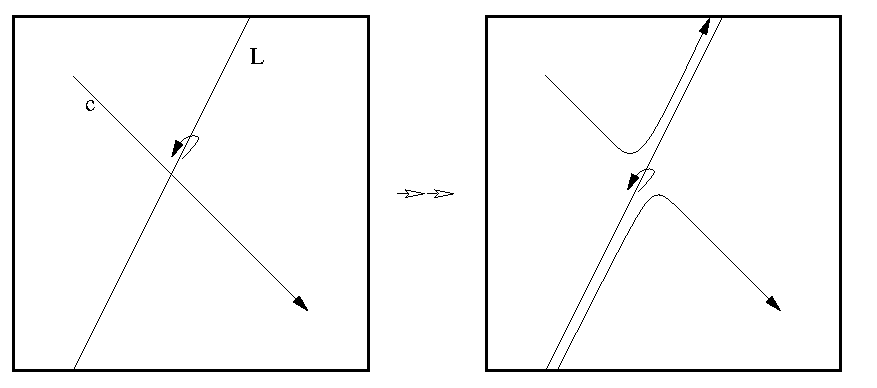
\includegraphics[width=0.62\textwidth]{figures/fig1.pdf}
  \caption{狄拉克弦与磁单极的磁场位形。(a) 磁荷 $g$ 位于原点，其磁场 $\vec{B}_{\rm mon}$ 沿径向向外；
           实心双线为狄拉克弦，其上携带回流磁通 $\vec{B}_{\rm sol}$。(b) 围绕狄拉克弦的闭合回路 $\Gamma$，
           用于计算沿回路的相位 $e\oint_\Gamma \vec{A}\cdot\mathrm{d}\vec{l}=eg$。原文仅标
           “Figure 1”（原文 PDF 第 7 页），无说明性图注；图注说明为译者据图补写。}
  \label{fig:1}
\end{figure}

\subsection{Georgi–Glashow 模型：一个有磁单极的简单理论}

到目前为止，我们一直在粒子力学的框架内工作，其中电荷与磁荷都是点状客体，并且是人为地引入理论中的。然而在场论中，这类客体也可以作为孤立子出现，即具有局域能量密度的场方程的非平凡解。如果与某孤立子解相联系的规范场位形具有磁性，该孤立子便可被认定为磁单极。最简单的孤立子出现在 Sine-Gordon 理论中，这是一个 $1+1$ 维的标量场论。然而，由 Derrick 定理，二维以上的标量场论不能支持静态有限能量解。这基本上是因为：孤立子在远距离处的非平凡结构使该位形的总能量发散。向理论中加入规范场可以弥补这一状况。因此，四维中含规范相互作用的标量理论可以容许静态有限能量的场位形。这类孤立子位形的稳定性往往与它们由守恒的拓扑荷所刻画这一事实有关。关于这些问题的更详细讨论，读者可参阅 \cite{GO, coleman1, coleman2}。下面我们描述 Georgi–Glashow 模型，这是一个 $3+1$ 维的、具有磁单极解的简单理论。

% [Tutor Note: 见原文 PDF 第 8 页“Derrick 定理”一句。原文只给结论，其证明是标度论证：对静态场作标度变换 $\phi_\lambda(\vec{x})=\phi(\lambda\vec{x})$，能量泛函可写成 $E(\lambda)=\lambda^{2-d}K+\lambda^{-d}V$（$K$ 为梯度项、$V$ 为势能项，均非负）；$d>1$ 时 $\mathrm{d}E/\mathrm{d}\lambda=0$ 无解，故 $d\ge2$ 的标量场论不存在静态有限能量解。原文另把这归因于孤立子在远距离处的非平凡结构，这是从位形角度的直观说法。]

Georgi–Glashow 模型是一个 Yang–Mills–Higgs 系统，它包含一个希格斯多重态 $\phi^a\,(a=1,2,3)$，它在规范群 $SO(3)$ 的伴随表示中按矢量变换，以及规范场 $W_\mu=W^a_\mu T^a$。这里，$T^a$ 是 $SO(3)$ 的厄米生成元，满足 $[T^a,T^b]=if^{abc}T^c$。在伴随表示中，有 $(T^a)_{bc}=-if^a_{bc}$；并且对 $SO(3)$ 而言 $f^{abc}=\epsilon^{abc}$。$W_\mu$ 的场强以及作用在 $\phi^a$ 上的协变导数定义为
\begin{eqnarray}
G_{\mu \nu} &=& \partial_{\mu}W_{\nu} - \partial_{\nu} W_{\mu} +
ie [W_{\mu},W_{\nu}]\,,
\nonumber\\
D_\mu\phi^a &=& \partial_\mu\phi^a - e\epsilon^{abc} W^b_\mu \phi^c\,.
\end{eqnarray}
最小拉格朗日量则为
\begin{equation}
{\cal L}  =  - \frac{1}{4} G^{a}_{\mu \nu} G^{a \mu \nu} +
\frac{1}{2} D^{\mu}\phi^a D_{\mu}\phi^a - V(\phi)\,,
\label{GGmodel}
\end{equation}
其中
\begin{equation}
V(\phi)=\frac{\lambda}{4}\left(\phi^2 - a^2 \right)^2\,.
\label{GGpot}
\end{equation}
由此拉格朗日量得到的运动方程为
\begin{equation}
(D_\nu G^{\mu \nu})^a=-e\,\epsilon^{abc}\,\phi^b\,(D^\mu\phi)^c,
\qquad D^\mu D_\mu \phi^a =-\lambda\phi^a (\phi^{2} - a^{2})\,. 
\label{XXIX}
\end{equation}
场强还满足比安基恒等式
\begin{equation}
D_\nu\,\widetilde G^{\mu \nu a} = 0\,.
\label{bianchi}
\end{equation}

% [Tutor Note: 见原文 PDF 第 8 页式 (15)、(16)。$W_\mu=W^a_\mu T^a$ 是矩阵值场，$G_{\mu\nu}=G^a_{\mu\nu}T^a$；用 $(T^a)_{bc}=-if^a_{bc}$ 与 $f^{abc}=\epsilon^{abc}$ 展开 $ie[W_\mu,W_\nu]$，得 $G^a_{\mu\nu}=\partial_\mu W^a_\nu-\partial_\nu W^a_\mu-e\epsilon^{abc}W^b_\mu W^c_\nu$。式中的因子 $i$ 与 $D_\mu\phi^a$ 里的 $-e$ 是配套的，符号弄反会直接改变式 (18) 的运动方程，并影响后文 BPS 界与磁荷的符号。]

我们来求该理论的真空位形。采用记号 $G_a^{0i}=-{\cal E}_a^i$ 与 $G_a^{ij} = -\epsilon^{ij}_
{\hphantom{ij}k}{\cal B}_a^k$，能量密度可写为
\begin{equation}
\theta_{00}=\frac{1}{2}\left(({\cal E}_a^i)^2+({\cal B}_a^i)^2 +
  (D^0\phi_a)^2 + ( D^i \phi_a)^2 \right) + V (\phi)\,.
\label{XXX}
\end{equation} 
注意 $\theta_{00} \geq 0$，并且它仅当下式成立时才为零：
\begin{equation}
G_{a}^{\mu \nu} = 0, \quad D_{\mu} \phi = 0, \quad V(\phi) = 0\,.
\label{XXXI}
\end{equation} 
第一个方程表明，在真空中 $W^a_\mu$ 是纯规范；后两个方程则定义了希格斯真空。真空空间的结构由 $V(\phi)=0$ 决定，其解为 $\phi^a= \phi^a_{vac}$，并满足 $|\phi_{vac}|=a$。因此，希格斯真空空间是场空间中半径为 $a$ 的二维球面（$S^2$）。为建立微扰论，我们必须选定其中一个真空，从而自发地破缺规范对称性（这就是通常的希格斯机制）。保持该真空不变的那部分对称性仍然保留下来，相应的未破缺生成元为 $\phi^c_{vac} T^c/a$。与该生成元相联系的规范玻色子是 $A_\mu=\phi^c_{vac}W^c_\mu/a$，而这一残存 $U(1)$ 的电荷算符由下式给出
\begin{equation} 
Q = \hbar e \frac{\phi^c_{vac}T^c}{a}\,.
\label{XXXIII}
\end{equation}
若群是紧致的，则该电荷是量子化的。理论的微扰谱可通过将 $\phi^a$ 在所选真空附近展开而得到：
$$
\phi^{a} = \phi^{a}_{vac} + \phi '^{a}\,.
$$
一个方便的选择是 $\phi^c_{vac}=\delta^{c3}a$。微扰谱（在选定适当规范后即显现）由一个有质量的希格斯粒子（$H$）、一个无质量光子（$\gamma$）和两个带电荷的有质量玻色子（$W^\pm$）组成；下表自左至右依次给出质量、自旋与电荷：
$$
\begin{tabular}{|c|c|c|c|}
\hline
& Mass & Spin & Charge \\
\hline
$H$ & $a(2\lambda)^{\frac{1}{2}} \hbar$ & $0$ &$0$ \\
\hline
$\gamma$ & $0$ & $\hbar$ & $0$ \\
\hline
$W^{\pm}$ & $ae\hbar = aq$ & $\hbar$ & $\pm q = \pm e \hbar$ \\
\hline
\end{tabular}
$$
下一节我们将考察 Georgi–Glashow 模型中磁单极（非微扰态）的存在性。

% [Tutor Note: 见原文 PDF 第 9 页微扰谱表格。表中“Spin”一列对光子与 $W^\pm$ 填 $\hbar$、对 $H$ 填 $0$，这是原文的写法：自旋一栏理应填自旋量子数 $1,1,0$（即 $s\hbar$ 中的 $s$），原文直接填入 $\hbar$，单位上亦不自洽，属原文笔误；为与源公式块保持一致，表头 Mass/Spin/Charge 保留原文，译名即“质量/自旋/电荷”。表中 $W^\pm$ 的质量 $ae\hbar=aq$ 与电荷 $\pm q=\pm e\hbar$ 彼此一致。]

% [Tutor Note: 本片原文拼写笔误汇总（译文均按正确词义翻译，源文件未改）：p2 “intented”→intended；p3 “proporties”→properties、“Minkowsky”→Minkowski；p4 “quations”→equations；p5 “elecromagnetic”→electromagnetic；p6 “fermios”→fermions，且“both of the components are bosonic.”句首小写；p7 “intruduced”→introduced；p8 “satifying”→satisfying、“representaion”→representation、“cavariant”→covariant。另有句读笔误一处，见式 (10) 前的批注。]
